\documentclass[conference, twoside]{IEEEtran}

\usepackage{tikz}
\newcommand{\onethird}{2.333333333cm}

\usetikzlibrary{positioning,fit,matrix}
\tikzstyle{architecture_node_nofill}=[rectangle, draw, minimum height=1cm,anchor=north west]
\tikzstyle{architecture_node_fullwidth}=[architecture_node_nofill,minimum width=7cm]
\tikzstyle{architecture_box}=[draw=black,dashed,anchor=north west]
\tikzstyle{architecture_no_fill}=[fill=none] % To disable all fills
\usetikzlibrary{calc, shapes.misc}

\usepackage{csvsimple}
\usepackage{amssymb}

% \newcommand\def{\stackrel{\mathclap{\normalfont\mbox{def}}}{=}}

\definecolor{lightred}{HTML}{EA2424}
\definecolor{red}{HTML}{D0021B}
\definecolor{lightblue}{HTML}{7D9FC7}
\definecolor{blue}{HTML}{4A90E2}
\definecolor{purple}{HTML}{7571A1}
\definecolor{green}{HTML}{70A500}
\definecolor{lightgreen}{HTML}{C1FF7D}
\definecolor{lightyellow}{HTML}{F8E71C}
\definecolor{yellow}{HTML}{F5A623}
\definecolor{lightorange}{HTML}{F56023}
\definecolor{orange}{HTML}{EB4400}
\definecolor{waterblue}{HTML}{6BE4C9}

\usepackage{multirow}

\usepackage[binary-units=true]{siunitx}

\usepackage{cite}

\usepackage[font={it}]{caption}
\captionsetup[figure]{name={Figure},labelsep=period}
\captionsetup[table]{name={Table},labelsep=period}
\usepackage{subcaption}

\usepackage{amsmath}
\usepackage[colorlinks]{hyperref}
\hypersetup{citecolor=black}
\hypersetup{linkcolor=black}
\hypersetup{urlcolor=black}
\usepackage{cleveref}
\usepackage{fancyvrb}

% format citations
\renewcommand\citepunct{, }
\renewcommand\citeleft{[}
\renewcommand\citeright{]}
\renewcommand\citedash{--}


\begin{document}
    % TITLE & PUBLICATION ID

    \title{An effective approach to steel defect detection} %  on steel surfaces
    \IEEEpubid{0000--0000/00\$00.00 ̃\copyright ̃2019 IEEE }

    % AUTHORS

    \author{
        \IEEEauthorblockN{Antonio Terpin}
        \IEEEauthorblockA{Electronic Engineering, Scuola Superiore\\
        Università degli Studi di Udine\\
        Udine, Italia \\
        Email: terpin.antonio@spes.uniud.it}
        \and
        \IEEEauthorblockN{Claudio Verardo}
        \IEEEauthorblockA{Electronic Engineering, Scuola Superiore\\
        Università degli Studi di Udine\\
        Udine, Italia \\
        Email: verardo.claudio@spes.uniud.it}
    }

    \maketitle
    \thispagestyle{plain}
    \pagestyle{plain}

    \begin{abstract}
    Quality control is a main issue in any industry. The need of assuring a human-like evaluation during products quality control has resulted in an active research aiming to develop an automatic defect detection scheme.
    In this paper an effective solution to defect detection on steel surfaces from images is presented. Firstly, a preprocessing step aiming to spot plausible defective areas is discussed. Lastly, the classification of these proposed regions is made. Hence, a proper segmentation scheme is described. Incidentally, a novel usage of the dilation factor in convolutional layers is introduced, providing an effective approach to classifying images of different sizes.
\end{abstract}

\begin{IEEEkeywords}
    Defect Detection, Computer Vision, Deep Learning, Wavelet.
\end{IEEEkeywords}
    % Introduction
    \section{Introduction}
    \begin{frame}{Introduction}
        \begin{abstract}
            Quality control is a main issue in any industry, and the automation of quality control process has become a hot topic in research. In this paper an effective solution to defect detection on steel surfaces from images is presented.
        \end{abstract}
        \vskip 0.5cm
        \begin{description}
            \item<1->[1.] Case study
            \item<2->[2.] Wavelet
            \item<3->[3.] Computer vision
        \end{description}
    \end{frame}
    % \subsection{Wavelet Analysis}
    \framepic{graphics/wavelets/wavelet}{
        \framefill
        \textcolor{black}{Wavelet}
        \vskip 0.5cm
    }

    \begin{frame}{Multi Resolution Analysis}
        \centering
        \onslide <1-> {
            \begin{block}{Goal}
                Approximate vectors of $L^2\left(\mathbb{R}\right)$ with variable degrees of resolution.
            \end{block}
        }
        \only <2> {
            \includegraphics[width=.6\textwidth]{graphics/wavelets/mra}
        }
        \only <3> {
            \includegraphics[width=.6\textwidth]{graphics/wavelets/mra-1}
        }
        \only <4> {
            \includegraphics[width=.6\textwidth]{graphics/wavelets/mra-2}
        }
        \only <5> {
            \includegraphics[width=.6\textwidth]{graphics/wavelets/mra-3}
        }
    \end{frame}

    \begin{frame}{Multi Resolution Analysis}
        \begin{block}{Axioms}
            \begin{equation}
                \cdots \subset V_{-2} \subset V_{-1} \subset V_0 \subset V_1 \subset V_2 \subset \cdots
            \end{equation}
            \begin{equation}
                \overline{\bigcup\limits_{n \in \mathbb{Z}} V_n} = L^2\left(\mathbb{R}\right)
            \end{equation}
            \begin{equation}
                \bigcap\limits_{n \in \mathbb{Z}} V_n = \left\{0\right\}
            \end{equation}
            \begin{equation}
                V_{n+1} = \mathcal{S}V_n
            \end{equation}
            \begin{equation}
                V_0 = \langle \left\{\tau^i\phi, i \in \mathbb{Z}\right\} \rangle \quad \exists \phi \in L^2\left(\mathbb{R}\right)\rangle
            \end{equation}
        \end{block}
    \end{frame}

    \begin{frame}{Multi Resolution Analysis}
        \begin{block}{Scaling function}
            \begin{equation}
                V_1 \supset V_0, \phi \in V_1
            \end{equation}
            \begin{equation}
                \left\{\mathcal{S}\tau^i\phi = \tau^{i/2}\mathcal{S}\phi, i \in \mathbb{Z}\right\} \; \text{orthonormal basis of } V_1
            \end{equation}
            \begin{equation}
                    \phi = \sum_{i \in \mathbb{Z}} g_i \tau^{i/2} \mathcal{S} \phi
            \end{equation}
        \end{block}
    \end{frame}

    \begin{frame}{Multi Resolution Analysis}
        \begin{block}{Wavelet}
            \begin{equation}
                V_{n+1} \supset V_n \Rightarrow \exists W_n \colon V_{n+1} = V_n \oplus W_n
            \end{equation}
            \begin{equation}
                \left\{\tau^i\psi\right\}_{i \in \mathbb{Z}} = W_0
            \end{equation}
            \begin{equation}
                \psi = \sum_{i \in \mathbb{Z}} h_i \tau^{i/2}\mathcal{S}\phi\quad\psi \in V_1
            \end{equation}
            \begin{equation}
                \langle \psi, \tau^i \psi \rangle = \delta_i
            \end{equation}
            \begin{equation}
                \langle \tau^j\psi, \tau^i \phi \rangle = 0
            \end{equation}
        \end{block}
    \end{frame}

    \begin{frame}
        \frametitle{Multi Resolution Analysis}
        \framesubtitle{Filter banks}
        \centering 
        \begin{tikzpicture}
            % High res
            \node[anchor= west] (highres) at (0,0) {$V_{n+1}$};
            % Low res
            \node[rectangle, draw, anchor= west, minimum height=0.75cm, minimum width=1.5cm] (g) at (3,2) {g};
            \node[circle, draw, anchor= west] (downsampleg) at (6,2) {$\downarrow 2$};
            \node[anchor= west] (lowres) at (8,2) {$V_n$};
            % Details
            \node[rectangle, draw, anchor= west, minimum height=0.75cm, minimum width=1.5cm] (h) at (3,-2) {h};
            \node[circle, draw, anchor= west] (downsampleh) at (6,-2) {$\downarrow 2$};
            \node[anchor= west] (details) at (8,-2) {$W_n$};

            \draw[->] (1,0) -- (2,0) -- (2,2) -- (3,2);
            \draw[->] (1,0) -- (2,0) -- (2,-2) -- (3,-2);

            \draw[->] (4.5,2) -- (6,2);
            \draw[->] (4.5,-2) -- (6,-2);

            \draw[->] (7,2) -- (8,2);
            \draw[->] (7,-2) -- (8,-2);

        \end{tikzpicture}
    \end{frame}

    \begin{frame}
        \frametitle{Wavelet: Example application}
        \framesubtitle{Detect abrupt changes}

        \centering
        \vskip -1cm
        $$s_1(t) = 2\sin\left(2\pi 10f_0 t\right) + \sin\left(2\pi 50f_0 t\right) + 10\delta\left(t - \frac{1}{2f_0}\right)$$
        \only<1> {
            \includegraphics[height=0.6\textheight]{graphics/wavelets/signal1}
        }
        \only<2> {
            \begin{columns}[onlytextwidth]
                \column{0.5\textwidth}
                \includegraphics[width=\textwidth]{graphics/wavelets/detect-abrupt-changes-fft}
                \column{0.5\textwidth}
                \includegraphics[width=\textwidth]{graphics/wavelets/detect-abrupt-changes-cwt}
            \end{columns}
        }

    \end{frame}

    \begin{frame}
        \frametitle{Wavelet: Example application}
        \framesubtitle{Detect temporal trends}
        $$f_{s_2} = e^t;\quad s_2 = \sin\left(2*pi*f_{s_2}t\right)$$
        \begin{columns}[onlytextwidth]
            \column{0.5\textwidth}
            \only<1-2> {
                \includegraphics[width=\textwidth]{graphics/wavelets/frequency-signal-2}
            }
            \only<3-4> {
                \includegraphics[width=\textwidth]{graphics/wavelets/detect-pattern-fft}
            }
            \column{0.5\textwidth}
            \only<2> {
                \includegraphics[width=\textwidth]{graphics/wavelets/signal2}
            }
            \only<4> {
                \includegraphics[width=\textwidth]{graphics/wavelets/detect-pattern-cwt}
            }
        \end{columns}
        
    \end{frame}


    \subsection{Computer Vision}
    \framepic{graphics/computervision/computer-vision}{
        \framefill
        \textcolor{white}{Computer Vision}
        \vskip 0.5cm
    }
    \begin{frame}{Computer Vision}
        \begin{block}{Classification Task}
            To determine to which of a set of \textbf{categories} a given object belongs to.
        \end{block}
        \begin{columns}[onlytextwidth]
            \column{0.3\textwidth}
            \centering
            \includegraphics[width=\textwidth]{graphics/computervision/classification-image.jpeg}
            \onslide <2-> {
                \column{0.4\textwidth}
                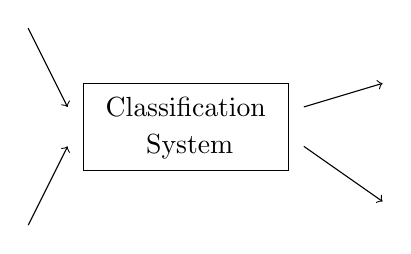
\begin{tikzpicture}
                    \node at (0,0) {Classification};
                    \node at (0.05,-0.5) {System};
                    \node[rectangle, draw, minimum width=2.6cm, minimum height=1.1cm, anchor=north west] at (-1.3,0.3) {};
                    \draw[->] (-2,1) -- (-1.5,0);
                    \draw[->] (-2,-1.5) -- (-1.5,-0.5);
                    \onslide <3-> {
                        \draw[->] (1.5,0) -- (2.5,0.3);
                        \draw[->] (1.5,-0.5) -- (2.5,-1.2);
                    }
                \end{tikzpicture}
            }
            \onslide <3-> {
                \column{0.2\textwidth}
                \vskip -0.5cm Output \vskip 0.5cm
                \begin{columns}[onlytextwidth]
                    \column{0.5\textwidth}
                        \begin{tabular}{|c|}
                            \hline
                            $0.03$\\\hline
                            \cellcolor{UniBlue}\textcolor{white}{$0.77$}\\\hline
                            $\vdots$\\\hline
                            $0.12$\\\hline
                        \end{tabular}
                    \column{0.5\textwidth}
                        \vskip -0.2cm
                        \begin{tabular}{c}
                            \\
                            \textcolor{UniBlue}{Child}\\
                            \\
                            \\
                        \end{tabular}
                \end{columns}
            }
        \end{columns}
    \end{frame}

    \begin{frame}{Computer Vision}
        \begin{block}{Object Localization Task}
            To find a given number (usually one) of items in a given context, predicting both their position and their class. \\
            \textbf{Remark.} Position is usually given as a bounding box.
        \end{block}
        \begin{columns}[onlytextwidth]
            \column{0.45\textwidth}
            \onslide <2-> {
                \includegraphics[width=\textwidth]{graphics/computervision/localization-input}
            }
            \column{0.45\textwidth}
            \onslide <3-> {
                \includegraphics[width=\textwidth]{graphics/computervision/localization-output}
            }
        \end{columns}
    \end{frame}

    \begin{frame}{Computer Vision}
        \onslide<1-> {
            \begin{block}{Object Detection Task}
                To \textbf{localize} any number of items in a given context, allowing either zero or any finite number of objects.
            \end{block}
        }
        \onslide<2-> {
            \begin{alertblock}{Remark.}
                The constraint on the number of object is \emph{a priori}. Indeed, a localization system will always look for a fixed number of objects, whereas a detection system is trained to be able to spot a variable number of objects in each input.
            \end{alertblock}
        }
    \end{frame}

    \begin{frame}{Computer Vision}
        \onslide <1-> {
            \begin{block}{Image Segmentation}
                Pixel-wide classification of the image. \textbf{Remark.} Image segmentation can be consider either the preemptive step to classification or the output of a classification system.
            \end{block}
        }
        \onslide <2-> {
            \vskip -0.5cm 
            \begin{exampleblock}{Example: Pixel-based image segmentation.}
                This family considers some distance defined over the image domain to segmentate it.
            \end{exampleblock}
        }
        \onslide <3-> {
            \vskip -0.5cm 
            \begin{exampleblock}{Example: Edge-based image segmentation.}
                This family uses an edge-detector algorithm, along with denoising and thresholding considerations, to solve the boundary detection problem.
            \end{exampleblock}
        }
    \end{frame}

    % \begin{frame}
    %     \frametitle{Pixel-based image segmentation}
    %     \framesubtitle{Whatershed}
    %     \begin{columns}[onlytextwidth]
    %         \column{0.5\textwidth}
    %         \includegraphics[width=\textwidth]{graphics/computervision/whatershed-plane}
    %         \column{0.5\textwidth}
    %         \includegraphics[width=\textwidth]{graphics/computervision/whatershed-surf}
    %     \end{columns}
    %     \only <1> {
    %         \begin{block}{Whatershed and immersion}
    %             The above pictures both show the same function defined over a 2D domain. Suppose to immerse the above right surface in some liquid, which gradually fill the two holes.
    %         \end{block}
    %     }
    %     \only <2> {
    %         \begin{block}{Whatershed and immersion}
    %             At some point the two volumes of liquid will meet, in particular they will flood at the same time over the green colored surface region.
    %         \end{block}
    %     }
    %     \only <3> {
    %         \begin{block}{Whatershed and immersion}
    %             This region is called whatershed and differentiates two areas of the image. Hence, an image can be segmentated considering its whatersheds.
    %         \end{block}
    %     }
    % \end{frame}

    % \begin{frame}
    %     \frametitle{Pixel-based image segmentation}
    %     \framesubtitle{Whatershed}
    %     % \includegraphics[width=\textwidth]{graphics/whatershed-plane}
    %     TODO insert example image\\
    %     % \includegraphics[width=\textwidth]{graphics/whatershed-surf}
    %     TODO insert example image
    % \end{frame}

    % \begin{frame}
    %     \frametitle{Pixel-based image segmentation}
    %     \framesubtitle{Whatershed}
    %     Let $\mathcal{D} \subset \mathbb{R}_+^2$ be a $2D$ domain, and $\mathcal{I} \colon \mathcal{D} \rightarrow \mathbb{R}_+$. Denote $\displaystyle h_m \triangleq \min_{\underline{x} \in \mathcal{D}}\mathcal{I}(\underline{x})$, $\displaystyle h_M \triangleq \max_{\underline{x} \in \mathcal{D}}\mathcal{I}(\underline{x})$, $T_h\left(\mathcal{I}\right) \triangleq \left\{\underline{p} \in \mathcal{D}, \mathcal{I}(\underline{p}) \leq h\right\}$.
    % \end{frame}

    % \begin{frame}
    %     \frametitle{Pixel-based image segmentation}
    %     \framesubtitle{Whatershed}
    %         \begin{itemize}
    %             \item Def, th, alg
    %             \item Example results
    %         \end{itemize}
    % \end{frame}
    \subsection{Deep Learning}
    \framepic{graphics/deeplearning/deep-learning}{
        \framefill
        \textcolor{white}{Deep Learning}
        \vskip 0.5cm
    }

    \begin{frame}{Computer Vision}
        \begin{block}{Classification Task}
            To determine to which of a set of \textbf{categories} a given object belongs to.
        \end{block}
        \begin{columns}[onlytextwidth]
            \column{0.3\textwidth}
            \centering
            \includegraphics[width=\textwidth]{graphics/computervision/classification-image.jpeg}
            \onslide <2-> {
                \column{0.4\textwidth}
                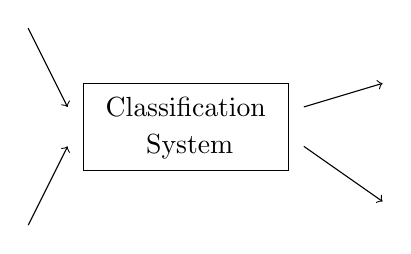
\begin{tikzpicture}
                    \node at (0,0) {Classification};
                    \node at (0.05,-0.5) {System};
                    \node[rectangle, draw, minimum width=2.6cm, minimum height=1.1cm, anchor=north west] at (-1.3,0.3) {};
                    \draw[->] (-2,1) -- (-1.5,0);
                    \draw[->] (-2,-1.5) -- (-1.5,-0.5);
                    \onslide <3-> {
                        \draw[->] (1.5,0) -- (2.5,0.3);
                        \draw[->] (1.5,-0.5) -- (2.5,-1.2);
                    }
                \end{tikzpicture}
            }
            \onslide <3-> {
                \column{0.2\textwidth}
                \vskip -0.5cm Output \vskip 0.5cm
                \begin{columns}[onlytextwidth]
                    \column{0.5\textwidth}
                        \begin{tabular}{|c|}
                            \hline
                            $0.03$\\\hline
                            \cellcolor{UniBlue}\textcolor{white}{$0.77$}\\\hline
                            $\vdots$\\\hline
                            $0.12$\\\hline
                        \end{tabular}
                    \column{0.5\textwidth}
                        \vskip -0.2cm
                        \begin{tabular}{c}
                            \\
                            \textcolor{UniBlue}{Child}\\
                            \\
                            \\
                        \end{tabular}
                \end{columns}
            }
        \end{columns}
    \end{frame}

    \begin{frame}{Computer Vision}
        \begin{block}{Object Localization Task}
            To find a given number (usually one) of items in a given context, predicting both their position and their class. \\
            \textbf{Remark.} Position is usually given as a bounding box.
        \end{block}
        \begin{columns}[onlytextwidth]
            \column{0.45\textwidth}
            \onslide <2-> {
                \includegraphics[width=\textwidth]{graphics/computervision/localization-input}
            }
            \column{0.45\textwidth}
            \onslide <3-> {
                \includegraphics[width=\textwidth]{graphics/computervision/localization-output}
            }
        \end{columns}
    \end{frame}

    \begin{frame}{Computer Vision}
        \onslide<1-> {
            \begin{block}{Object Detection Task}
                To \textbf{localize} any number of items in a given context, allowing either zero or any finite number of objects.
            \end{block}
        }
        \onslide<2-> {
            \begin{alertblock}{Remark.}
                The constraint on the number of object is \emph{a priori}. Indeed, a localization system will always look for a fixed number of objects, whereas a detection system is trained to be able to spot a variable number of objects in each input.
            \end{alertblock}
        }
    \end{frame}

    \begin{frame}{Computer Vision}
        \onslide <1-> {
            \begin{block}{Image Segmentation}
                Pixel-wide classification of the image. \textbf{Remark.} Image segmentation can be consider either the preemptive step to classification or the output of a classification system.
            \end{block}
        }
        \onslide <2-> {
            \vskip -0.5cm 
            \begin{exampleblock}{Example: Pixel-based image segmentation.}
                This family considers some distance defined over the image domain to segmentate it.
            \end{exampleblock}
        }
        \onslide <3-> {
            \vskip -0.5cm 
            \begin{exampleblock}{Example: Edge-based image segmentation.}
                This family uses an edge-detector algorithm, along with denoising and thresholding considerations, to solve the boundary detection problem.
            \end{exampleblock}
        }
    \end{frame}

    \begin{frame}{Training}
        \begin{block}{Forward propagation}
            The \emph{feedforward} neural network accepts an input $\underline{\underline{X}}$ and produce an output $\underline{y}$. The information from $\underline{\underline{X}}$ flows through the hidden units to produce $\underline{y}$. This is called \textbf{forward propagation}.
        \end{block}

        \begin{block}{Backward propagation}
            During the training the forward propagation can continue onward to evaluate a scalar cost $J\left(\underline{\underline{\theta}}\right)$. The \textbf{back-propagation} algorithm is a numerically efficient way to compute cost gradient, in order to perform gradient descent.
        \end{block}    
    \end{frame}

    \begin{frame}{Deep Learning}
        \includegraphics[width=\textwidth]{graphics/deeplearning/nn}
    \end{frame}

    \begin{frame}
        \frametitle{Training}
        \framesubtitle{Backpropagation (proof)}
        \centering
        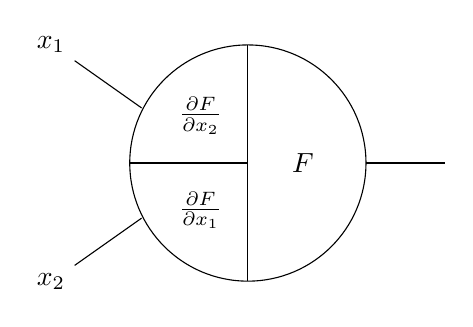
\begin{tikzpicture}
            \node[circle, draw, minimum width=3cm, minimum height=3cm] at (0,0) {};
            \node at (0.7,0) {$F$};
            \node at (-0.6,-0.6) {$\frac{\partial F}{\partial x_1}$};
            \node at (-0.6,0.6) {$\frac{\partial F}{\partial x_2}$};
            \node at (-2.5,1.5) {$x_1$};
            \node at (-2.5,-1.5) {$x_2$};

            \draw (0,0) -- (-1.5,0);
            \draw (0,-1.5) -- (0,1.5);
            \draw (1.5, 0) -- (2.5,0);

            \draw (-1.35, 0.7) -- (-2.2,1.3);
            \draw (-1.35, -0.7) -- (-2.2,-1.3);
        \end{tikzpicture}

        \vskip 0.5cm
        
        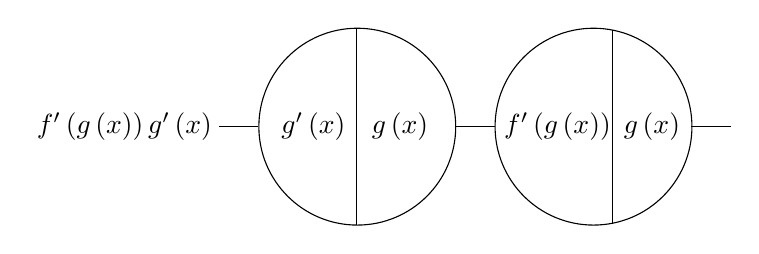
\begin{tikzpicture}
            \node at (-.7,0) {$f'\left(g\left(x\right)\right)g'\left(x\right)$};

            \draw (0.5,0) -- (1,0);

            \node[circle, draw, minimum width=2.5cm, minimum height=2.5cm, anchor=west] at (1,0) {};
            \node at (1.7, 0) {$g'\left(x\right)$};
            \node at (2.8, 0) {$g\left(x\right)$};
            \draw (2.25, 1.25) -- (2.25, -1.25);

            \draw (3.5, 0) -- (4, 0);

            \node[circle, draw, minimum width=2.5cm, minimum height=2.5cm, anchor=west] at (4,0) {};
            \node at (4.8, 0) {$f'\left(g\left(x\right)\right)$};
            \node at (6, 0) {$g\left(x\right)$};
            \draw (5.5, 1.23) -- (5.5, -1.23);

            \draw (6.5, 0) -- (7, 0);

        \end{tikzpicture}
    \end{frame}

    \begin{frame}{Convolutional Networks}
        \includegraphics[width=\textwidth]{graphics/deeplearning/cnn}
        \vskip 0.5cm
        \begin{exampleblock}{Motivation}
            \begin{enumerate}
                \item Sparse interactions
                \item Parameter sharing
                \item Equivariant representations
                \item Biologically inspired artificial intelligence
            \end{enumerate}
        \end{exampleblock}
    \end{frame}

    \begin{frame}{Convolutional Networks}
        \includegraphics[width=\textwidth]{graphics/deeplearning/cnn}
        \onslide <1-> {
            \begin{block}{Convolutional neural networks (CNN)}
                CNNs are a specialized kind of neural network for processing data that has a known grid-like topology.
            \end{block}
        }
        \onslide <2-> {
            \begin{block}{Convolutional neural networks (CNN) - 2}
                CNNs are neural networks that use convolution in place of general matrix multiplication in at least one of their layers.
            \end{block}
        }
    \end{frame}


    \section{Steel surfaces defect detection}
    \subsection{Problem statement}
        \par{
            \emph{Given a set of steel surfaces images with the description of their defective areas, learn to detect defective pixels in new pictures.}
        }
        \begin{figure}
            \includegraphics[width=\linewidth]{graphics/architecture/architecture-input}
            \vskip .05cm
            \includegraphics[width=\linewidth]{graphics/architecture/architecture-output}
            \caption{Detection process input and output.}\label{fig:exampledetection}
        \end{figure}
        \par{
            The surfaces may have more disjunct defective areas, and there are four defective classes, described in \ref{subsection:defects}.
        }
        \par{
            For each of this areas, a thorough characterization of the member pixels must be provided, along with the class of the defect pictured in the considered region.
        }
        \par{
            Defective pixels are described using a Run Length Encoding (RLE) approach. The rationale is that an efficient way to store pixel-wide information is needed, and it is reasonable to believe that many defective pixels will be adjacent.
        }
        \par{
            To do so, the binary matrix describing interesting pixels is firstly vectorized column-wide, i.e. each column vector is appended to the previous.
        }
        \par{
            Secondly, pixels are enumerated in this vectorized map.
        }
        \par{
            Finally, the rle algorithm is used on the indices of the cosidered pixels.
        }
        \par{
            \begin{BVerbatim}

Example:

    Suppose the ones in the below 
    matrix need to be encoded:
     _       _
    | 1 0 1 1 |
    | 1 1 1 0 |
    | 0 1 1 0 |
     -       -

    The interested cells, expressed 
    as (x, y) coordinates, are:

    [(1, 1) (1, 2) (2, 2) (2, 3)
        (3, 1) (3, 2) (3, 3) (4, 1)]
    
    The vectorized matrix is:

    [1 1 0 0 1 1 1 1 1 1 0 0]

    Which can be encoded as:

    "1 2 4 6"
           
            \end{BVerbatim}
        }
        \par{
            An optimized implementation in \texttt{MATLAB} of both the rle encoding and decoding scheme described is proposed in \cite{antonioterpin:github}.
        }
        \par{
            A visual description of the end to end process is given in figure \ref{fig:exampledetection}, where defective areas have been highlighted with different colors, depending on the defect class.
        }
        \par{
            A mathematical description of the task is:
        }
        \par{
            Given a \emph{training set} $\left(\underline{\underline{\mathbf{X}}}_{train}, \underline{\mathbf{y}}_{train}\right)$ and a \emph{test set} $\left(\underline{\underline{\mathbf{X}}}_{test}, \underline{\mathbf{y}}_{test}\right)$, the goal is to build a \emph{trainer} system $\mathcal{T}$ and a \emph{predictor} function $\mathcal{P}$ such that:
            \begin{equation*}
                \underline{\underline{\mathbf{\Theta}}} = \mathcal{T}\left(\underline{\underline{\mathbf{X}}}_{train}, \underline{\mathbf{y}}_{train}\right);\quad \lvert \mathcal{P}\left(\underline{\underline{\mathbf{X}}}_{test}; \underline{\underline{\mathbf{\Theta}}}\right) - \underline{\mathbf{y}}_{test} \rvert \rightarrow 0
            \end{equation*}
        }
        \par{
            Both the trainer and the predictor are implemented through deep learning tecniques and they are described in \ref{section:architecture}.
        }

    \subsection{Defect analysis}\label{subsection:defects}
        \par{
            The dataset is concerned with flat steel sheet, which production process is especially delicate and structured in many phases.
        }
        \par{
            Therefore, there are numerous defects classified in literature \cite{defects:64common,defects:mainlinemetals}. Hence, many of the traditional types may have been grouped together in the four classes given. However, in this section a plausible explanation of each defect class is provided.
        }
        \par{
            The fundamental observation, however, is that some defects have a global origin, i.e. they are due to a flawed machinery, therefore is reasonable that a local classifier would miss some important details.
        }
        % \par{
        %     One of the main stage of the production process is rolling \cite{wiki:rolling, defects:rolling}, which is the procedure of plastically deforming steel by passing it between rolls. Therefore, the steel is subjected to high compressive stresses as a result of the friction between the rolls and the metal surface.
        % }
        % \par{
        %     The semi-finished products of casting are named \emph{bloom}, \emph{billet} and \emph{slab}. The former is the product of the first breakdown of the ingot, the second is obtained from a further reduction by hot rolling, and the latter is obtained by rolling the ingot or the bloom.
        % }
        % \par{
        %     Rolling mill products are called \emph{plate}, \emph{sheet}, \emph{strip} based on their size.
        % }
        % \par{
        %     The plate has a thickness greater then $\SI{6}{\mm}$, whereas both sheet and strip are smaller. However, the latters are distinguished by their width. Sheets width is larger then $\SI{600}{\mm}$, whereas strips width is not.
        % }
        \subsubsection{Defect class \#1}\label{section:defect-class-1}
            \par{
                The first type of defect has not been classified yet into one of the classes found in literature.
            }
            \begin{figure}
                \includegraphics[width=\linewidth]{graphics/defects/class1surface}
                \vskip .05cm
                \includegraphics[width=\linewidth]{graphics/defects/class1surface-highlighted}
                \caption{Steel surface with defect class \#1.}\label{fig:defects:surface-1}
            \end{figure}
            \begin{figure}
                \centering
                \includegraphics[width=\linewidth]{graphics/defects/nregions-class1}
                \caption{Number of defects of class 1 per defective surface.}\label{fig:nregions-1}
            \end{figure}
            \par{
                However, it is a glaring example of burst defect, indeed it is reasonable to expect such defect to repeat multiple times on the same surface, as deducible from the histogram in figure \ref{fig:nregions-1}.
            }
            \begin{figure}
                \includegraphics[width=\linewidth]{graphics/defects/class1shape}
                \caption{Shape distribution for defect class \#1.}\label{fig:defects:shape-1}
            \end{figure}
            \begin{figure}
                \centering
                \includegraphics[width=\linewidth]{graphics/defects/class1-height-distribution}
                % \includegraphics[width=\linewidth]{graphics/defects/class1-height-distribution-log}
                \includegraphics[width=\linewidth]{graphics/defects/class1-length-distribution}
                % \includegraphics[width=\linewidth]{graphics/defects/class1-length-distribution-log}
                % \includegraphics[width=\linewidth]{graphics/defects/class1-gaussian}
                \caption{Defect class \#1 dimensions distribution.}\label{fig:defects:gaussian-1}
            \end{figure}
            \par{
                An example of surface with a burst of class \#1 defects is visible in illustration \ref{fig:defects:surface-1}. The shape distribution of the defect is illustrated in picture \ref{fig:defects:shape-1}.
            }
            \par{
                This is drawn by super-position of all the defects of the same type, centered in the middle of the figure, and counting the relative frequencies of each pixel.
            }
            \par{
                Defect \#1 dimensions distribution is shown in \ref{fig:defects:gaussian-1}. 
            }
            \begin{table}
                \centering
                \begin{tabular}{|c|c|c|}
                    \hline
                    \textbf{Length distribution} & $p$-value & Null hypothesis rejected
                    \csvreader[head to column names]{data/lengthDistribution1.csv}{}% use head of csv as column names
                    {\\\hline\Distribution&\pValue&\h}% specify your coloumns here
                    \\\hline
                    \textbf{Height distribution} & $p$-value & Null hypothesis rejected
                    \csvreader[head to column names]{data/heightDistribution1.csv}{}% use head of csv as column names
                    {\\\hline\Distribution&\pValue&\h}% specify your coloumns here
                    \\\hline
                \end{tabular}
                \vspace{0.25cm}
                \caption{hypotheses test results on class \#1.}\label{table:hypotheses-test-1}
            \end{table}
            \par{
                In table \ref{table:hypotheses-test-1} are shown the results of some distribution hypothesis tests. The null hypotheses are data following a particular distribution (e.g. Lognormal, Normal, Weibull), with their parameters tuned using the best sample estimators. It is visible that it is not possible to infer the distribution, and it is eventually better to use a kernel distribution.
            }
            \par{
                Therefore, no information on the tuning of the architecture hyperparameters has been extrapolated from data distribution.
            }
        \subsubsection{Defect class \#2}\label{section:defect-class-2}
            \par{
                Defects of class \#2 usually appears near the transversal edge, hence, they are probably edge laminations, since they are also visually similar.
            }
            \begin{figure}
                \includegraphics[width=\linewidth]{graphics/defects/class2surface}
                \vskip .05cm
                \includegraphics[width=\linewidth]{graphics/defects/class2surface-highlighted}
                \caption{Steel surface with defect class \#2.}\label{fig:defects:surface-2}
            \end{figure}
            \begin{figure}
                \centering
                \includegraphics[width=\linewidth]{graphics/defects/nregions-class2}
                \caption{Number of defects of class 2 per defective surface.}\label{fig:nregions-2}
            \end{figure}
            \par{
                These defects are local, since they are usually near the edge. Indeed, from the histogram in figure \ref{fig:nregions-2} is visible that they occur only a small limited number of times on the same surface.
            }
            % \par{
            %     This defects are due to the overcooling of the slab off of the caster. The coil mill edges looks like a continuous or semi-continuous line of slivers.
            % }
            \begin{figure}
                \includegraphics[width=\linewidth]{graphics/defects/class2shape}
                \caption{Shape distribution for defect class \#2.}\label{fig:defects:shape-2}
            \end{figure}
            \begin{figure}
                \centering
                \includegraphics[width=\linewidth]{graphics/defects/class2-height-distribution}
                % \includegraphics[width=\linewidth]{graphics/defects/class2-height-distribution-log}
                \includegraphics[width=\linewidth]{graphics/defects/class2-length-distribution}
                % \includegraphics[width=\linewidth]{graphics/defects/class2-length-distribution-log}
                % \includegraphics[width=\linewidth]{graphics/defects/class2-gaussian}
                \caption{Defect class \#2 dimensions distribution.}\label{fig:defects:gaussian-2}
            \end{figure}
            \par{
                In figure \ref{fig:defects:surface-2} an example of surface with a defect of this type is shown. The shape distribution of the defect is illustrated in picture \ref{fig:defects:shape-2}.
            }
            \par{
                Defect \#2 dimensions distribution is shown in \ref{fig:defects:gaussian-2}. 
            }
            \begin{table}
                \centering
                \begin{tabular}{|c|c|c|}
                    \hline
                    \textbf{Length distribution} & $p$-value & Null hypothesis rejected
                    \csvreader[head to column names]{data/lengthDistribution2.csv}{}% use head of csv as column names
                    {\\\hline\Distribution&\pValue&\h}% specify your coloumns here
                    \\\hline
                    \textbf{Height distribution} & $p$-value & Null hypothesis rejected
                    \csvreader[head to column names]{data/heightDistribution2.csv}{}% use head of csv as column names
                    {\\\hline\Distribution&\pValue&\h}% specify your coloumns here
                    \\\hline
                \end{tabular}
                \vspace{0.25cm}
                \caption{hypotheses test results on class \#2.}\label{table:hypotheses-test-2}
            \end{table}
            \par{
                In table \ref{table:hypotheses-test-2} are shown the results of some distribution hypothesis tests. It is clear that it is not possible to model the height with any distribution, whereas the length may be modeled with the kernel distribution. 
            }
        \subsubsection{Defect class \#3}\label{section-defect-class-3}
            \par{
                The mill rolls should be perfectly parallel to correctly flatten the steel. When this is not the case, a stress pattern arises, with tension along the centreline.
            }
            \begin{figure}
                \includegraphics[width=\linewidth]{graphics/defects/class3surface}
                \vskip .05cm
                \includegraphics[width=\linewidth]{graphics/defects/class3surface-highlighted}
                \caption{Steel surface with defect class \#3.}\label{fig:defects:surface-3}
            \end{figure}
            \par{
                Defects of class \#3 are probably rolling defects, in particular their repetitive pattern along the centreline is a symptom of \emph{zipper cracks}, i.e. centre line cracking. This is another patent example of burst defect.
            }
            \begin{figure}
                \centering
                \includegraphics[width=\linewidth]{graphics/defects/nregions-class3}
                \caption{Number of defects of class 3 per defective surface.}\label{fig:nregions-3}
            \end{figure}
            \par{
                The hypothesis of transversality of the presence of a defect of class \#3 over the surface is supported by the histogram in figure \ref{fig:nregions-3}. However, as extrapolated from a visual analysis (as an example, consider figure \ref{fig:defects:surface-3}), many defects of class \#3 are encoded together, since they are very near one another. Hence, many of these are considered as an atomic region.
            }
            \begin{figure}
                \includegraphics[width=\linewidth]{graphics/defects/class3shape}
                \caption{Shape distribution for defect class \#3.}\label{fig:defects:shape-3}
            \end{figure}
            \begin{figure}
                \centering
                \includegraphics[width=\linewidth]{graphics/defects/class3-height-distribution}
                % \includegraphics[width=\linewidth]{graphics/defects/class3-height-distribution-log}
                \includegraphics[width=\linewidth]{graphics/defects/class3-length-distribution}
                % \includegraphics[width=\linewidth]{graphics/defects/class3-length-distribution-log}
                % \includegraphics[width=\linewidth]{graphics/defects/class3-gaussian}
                \caption{Defect class \#3 dimensions distribution.}\label{fig:defects:gaussian-3}
            \end{figure}
            \par{
                An example of surface affected by defects of class \#3 is shown in figure \ref{fig:defects:surface-3}. A single defect of class \#3 (i.e. a single crack) has usually the shape shown in picture \ref{fig:defects:shape-3}.
            }
            \par{
                Defect \#3 dimensions distribution is shown in \ref{fig:defects:gaussian-3}. 
            }
            \begin{table}
                \centering
                \begin{tabular}{|c|c|c|}
                    \hline
                    \textbf{Length distribution} & $p$-value & Null hypothesis rejected
                    \csvreader[head to column names]{data/lengthDistribution3.csv}{}% use head of csv as column names
                    {\\\hline\Distribution&\pValue&\h}% specify your coloumns here
                    \\\hline
                    \textbf{Height distribution} & $p$-value & Null hypothesis rejected
                    \csvreader[head to column names]{data/heightDistribution3.csv}{}% use head of csv as column names
                    {\\\hline\Distribution&\pValue&\h}% specify your coloumns here
                    \\\hline
                \end{tabular}
                \vspace{0.25cm}
                \caption{hypotheses test results on class \#3.}\label{table:hypotheses-test-3}
            \end{table}
            \par{
                In table \ref{table:hypotheses-test-3} are shown the results of some distribution hypothesis tests. Conclusions are the same discussed in \ref{section:defect-class-2}.
            }

        \subsubsection{Defect class \#4}\label{section-defect-class-4}
            \par{
                This defect class seems to be concerned with protrusions on the steel surface. The main typologies of protuberances in the given dataset are \emph{scabs} and \emph{blisters}.
            }
            \begin{figure}
                \includegraphics[width=\linewidth]{graphics/defects/class4surface}
                \vskip .05cm
                \includegraphics[width=\linewidth]{graphics/defects/class4surface-highlighted}
                \caption{Steel surface with defect class \#4.}\label{fig:defects:surface-4}
            \end{figure}
            \par{
                Scabs are flattened protrusions, and they tend to be round or oval shaped and concentrated to only certain blooms or billets.
            }
            \par{
                Blisters, or gas porosities, are small bulges on the surface of the components and their dimension can vary. Some gasses may remain trapped inside the steel sheet. The high pressure due to the rolling process produces then protrusions on the surface.
            }
            \begin{figure}
                \includegraphics[width=\linewidth]{graphics/defects/class4shape}
                \caption{Shape distribution for defect class \#4.}\label{fig:defects:shape-4}
            \end{figure}
            \begin{figure}
                \centering
                \includegraphics[width=\linewidth]{graphics/defects/class4-height-distribution}
                % \includegraphics[width=\linewidth]{graphics/defects/class4-height-distribution-log}
                \includegraphics[width=\linewidth]{graphics/defects/class4-length-distribution}
                % \includegraphics[width=\linewidth]{graphics/defects/class4-length-distribution-log}
                % \includegraphics[width=\linewidth]{graphics/defects/class4-gaussian}
                \caption{Defect class \#4 dimensions distribution.}\label{fig:defects:gaussian-4}
            \end{figure}
            \par{
                An example of surface affected by defects of class \#4 is shown in figure \ref{fig:defects:surface-4}. A single defect of class \#4 (i.e. a single crack) has usually the shape shown in picture \ref{fig:defects:shape-4}.
            }
            \par{
                Defect \#4 dimensions distribution is shown in \ref{fig:defects:gaussian-4}. 
            }
            \begin{table}
                \centering
                \begin{tabular}{|c|c|c|}
                    \hline
                    \textbf{Length distribution} & $p$-value & Null hypothesis rejected
                    \csvreader[head to column names]{data/lengthDistribution4.csv}{}% use head of csv as column names
                    {\\\hline\Distribution&\pValue&\h}% specify your coloumns here
                    \\\hline
                    \textbf{Height distribution} & $p$-value & Null hypothesis rejected
                    \csvreader[head to column names]{data/heightDistribution4.csv}{}% use head of csv as column names
                    {\\\hline\Distribution&\pValue&\h}% specify your coloumns here
                    \\\hline
                \end{tabular}
                \vspace{0.25cm}
                \caption{hypotheses test results on class \#4.}\label{table:hypotheses-test-4}
            \end{table}
            \par{
                In table \ref{table:hypotheses-test-4} are shown the results of some distribution hypothesis tests. Conclusions are the same discussed in \ref{section:defect-class-1}.
            }
            \begin{figure}
                \centering
                \includegraphics[width=\linewidth]{graphics/defects/nregions-class4}
                \caption{Number of defects of class 4 per defective surface.}\label{fig:nregions-4}
            \end{figure}
            \par{
                Even this defect class has global characteristics, as confirmed by the histogram in picture \ref{fig:nregions-4}.
            }
    \subsection{Dataset considerations}
        \begin{figure}
            \includegraphics[width=\linewidth]{graphics/defects/representation}
            \caption{Class representation in the original dataset.}\label{fig:defects:representation-original}
        \end{figure}
        \par{
            The dataset is composed by images linked to up to four strings of RLE encoded pixels, one per defect class.
        }
        \par{
            In illustration \ref{fig:defects:representation-original} the relative representation of the classes in the original dataset is shown. It is patent that class 3 is far more represented then the other defect classes, and the number of surfaces with at least a defect of this class is nearly tantamount the number of flawless surfaces.
        }
        \begin{figure}
            \includegraphics[width=\linewidth]{graphics/defects/combinations}
            \caption{Frequencies of defects combinations.}\label{fig:defects:combinations}
        \end{figure}
        \par{
            In figure \ref{fig:defects:combinations} images have been grouped in mutually exclusive subsets, based on the combination of defects in the pictured surface.
        }
        \par{
            Since skewed dataset lessen the effectiveness of machine learning algorithms, especially in predicting minority class examples, data augmentation is done only on those classes or combinations of classes with fewer elements.
        }
        \begin{figure}
            \includegraphics[width=\linewidth]{graphics/defects/data-augmentation}
            \vskip .05cm
            \includegraphics[width=\linewidth]{graphics/defects/data-augmentation-h}
            \vskip .05cm
            \includegraphics[width=\linewidth]{graphics/defects/data-augmentation-v}
            \vskip .05cm
            \includegraphics[width=\linewidth]{graphics/defects/data-augmentation-hv}
            \caption{Data augmentation. The image is flipped horizontally, vertically and both. The defective area is moved coherently.}\label{fig:data-augmentation}
        \end{figure}
        \par{
            In order to keep proper proportions and spatial information, replicas of surfaces are built only using simmetries. Therefore, from a single image other three are generated. An example of such operation is shown in \ref{fig:data-augmentation}.
        }
        \par{
            The encoded defective pixels must be mapped onto the new image. This can be easily done considering the binary matrix corresponding to the encoded pixels, flipping it and re-encoding the resulting map.
        }
        \begin{figure}
            \includegraphics[width=\linewidth]{graphics/defects/representation-augmented}
            \caption{Class representation in the augmented dataset.}\label{fig:defects:representation-augmented}
        \end{figure}
        \par{
            The resulting dataset is slightly more balanced. The bar chart in figure \ref{fig:defects:representation-augmented} shows the new representation of the different classes after data augmentation.
        }
    % Architecture
    \section{Architecture overview}\label{section:architecture}
    \begin{figure}
        \centering
        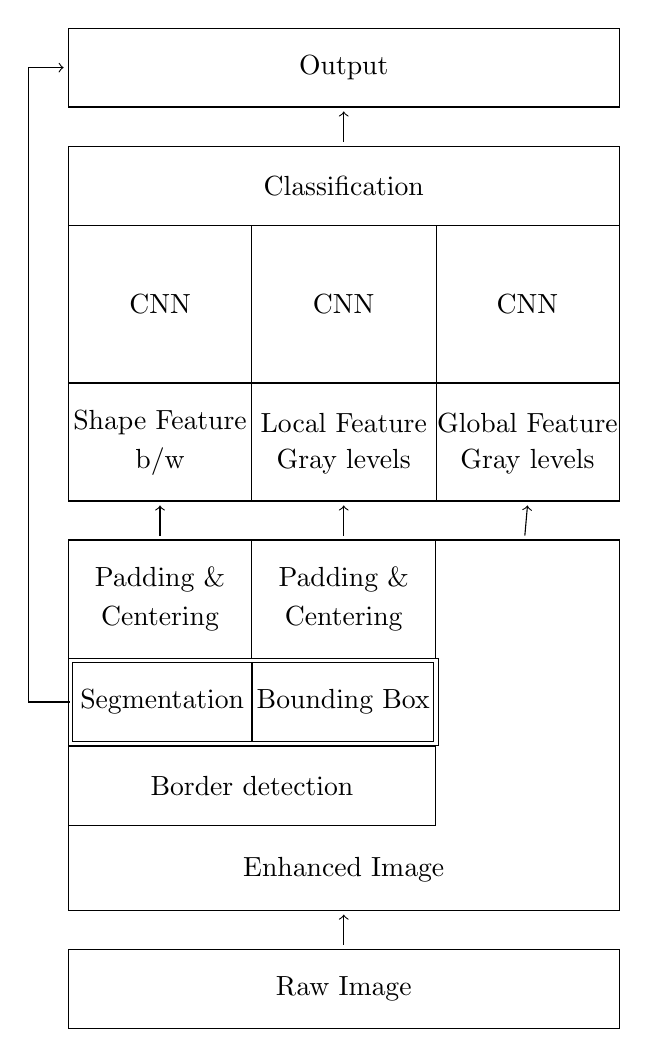
\begin{tikzpicture}

            % \draw[help lines] (0,0) grid (8.5,16);

            % Output
            \node[architecture_node_fullwidth,fill=waterblue,architecture_no_fill] (output) at (1,16) {Output};

            % Classificator
            % \node[architecture_box,minimum width=7.2cm,minimum height=4.7cm] (classification_architecture) at (.9,14.6) {};
            \node[architecture_node_fullwidth,fill=purple,architecture_no_fill] (classification) at (1,14.5) {Classification};
                    % CNN
                \matrix[architecture_node_nofill,minimum width=\onethird,minimum height=2cm,inner sep=0mm,fill=blue,architecture_no_fill] (cnn) at (1,13.5) {
                    \node {CNN}; & \node (cnn_local) {CNN}; & \node {CNN}; \\
                };
                \draw[black] (cnn_local.north east)--(cnn_local.south east);
                \draw[black] (cnn_local.north west)--(cnn_local.south west);

                    % INPUT
                \matrix[architecture_node_nofill,minimum width=\onethird,minimum height=1cm,inner sep=0mm,row sep=-0.51cm,fill=lightblue,architecture_no_fill] (cnn_features) at (1,11.5) {
                    \node (cnn_shape_feature) {Shape Feature}; & \node (cnn_local_feature) {Local Feature}; & \node (cnn_global_feature) {Global Feature}; \\
                    \node (cnn_shape_feature_color) {b/w}; & \node (cnn_local_feature_color) {Gray levels}; & \node (cnn_global_feature_color) {Gray levels}; \\
                };
                \draw[black] (cnn_local_feature.north east)--(cnn_local_feature_color.south east);
                \draw[black] (cnn_local_feature.north west)--(cnn_local_feature_color.south west);
            
            \draw[->] ($(classification.north) + (0,.05)$) -- ($(output.south) + (0,-0.05)$);

            % INPUT PREPROCESSING
                % Enhanced image
                \node[architecture_node_fullwidth,minimum height=4.7cm,fill=lightyellow,architecture_no_fill] (enhanced_image_box) at (1,9.5) {};
                \node[architecture_node_fullwidth,minimum height=1cm,anchor=south west,draw=none] (enhanced_image_label) at (1,4.8) {Enhanced Image};
                % \node[architecture_box,minimum width=7.2cm,minimum height=4.9cm] (preprocessing_architecture) at (.9,9.6) {};

                % Padding
                \matrix[architecture_node_nofill,minimum width=\onethird,minimum height=1cm,inner sep=0mm,row sep=-0.51cm,fill=lightred,architecture_no_fill] (cnn) at (1,9.5) {
                    \node (padding1) {Padding \&}; & \node (padding2) {Padding \&};\\
                    \node {Centering}; & \node (centering2) {Centering};\\
                };
                \draw[black] (padding2.north west)--(centering2.south west);

                % Segmentation & Bounding box
                \matrix[architecture_node_nofill,minimum width=\onethird - .6mm,minimum height=1cm,inner sep=.5mm,nodes={draw=black},fill=lightorange,architecture_no_fill,nodes={fill=orange,architecture_no_fill}] (segmentation_bounding_box) at (1,8) {
                    \node {Segmentation}; & \node {Bounding Box};\\
                };

                % Border detection & Region proposals
                \node[architecture_node_nofill,minimum width=2*\onethird,minimum height=1cm,fill=yellow,architecture_no_fill] (border) at (1,6.88) {Border detection};
            
            \draw[->] ($(segmentation_bounding_box.west) + (0.03,0)$) -- ($(segmentation_bounding_box.west) + (-0.5,0)$) -- ($(output.west) + (-0.5,0)$) -- ($(output.west) + (-0.05,0)$);
            \draw[->] ($(padding1.north) + (0,.05)$) -- ($(cnn_shape_feature_color.south) + (0,-0.05)$);
            \draw[->] ($(padding2.north) + (0,.05)$) -- ($(cnn_local_feature_color.south) + (0,-0.05)$);
            \draw[->] ($(enhanced_image_box.north) + (2.3cm,.05)$) -- ($(cnn_global_feature_color.south) + (0,-0.05)$);

            % Raw image
            \node[architecture_node_fullwidth,fill=green,architecture_no_fill] (rawim) at (1,4.3) {Raw Image};
            \draw[->] ($(rawim.north) + (0,.05)$) -- ($(enhanced_image_box.south) + (0,-0.05)$);

        \end{tikzpicture}
        \caption{Proposed defect detection system architecture}\label{fig:architecture}
    \end{figure}

    \par{
        The defect detection system architecture proposed in this paper is described in \emph{Figure \ref{fig:architecture}}.
    }

    \par{
        Steel surfaces pictures of $1600\times 256$ pixels are taken at the input of the process. Since they may be taken under different light exposure conditions, some preprocessing is made to enhance the quality of the image, e.g. histogram equalization or linear scaling. Moreover, the images considered have three equal colours levels, therefore they are converted into gray levels, to save space. This first step is further described in \emph{Section \ref{section:image_preprocessing}}.
    }
    \par{
        The aim of the architecture proposed in this paper is both to detect pixels representing steel imperfections and to classify those regions. Therefore, image segmentation is either obtained as an output of the system or it is needed in some step during the process. The latter situation can be achieved through a brute-force multi-scale sliding window, but to improve performances without reducing accuracy a particular implementation of a Region based CNN (R-CNN) \cite{ieee:7410526,ieee:7532516} is proposed in \emph{Section \ref{section:mc-cnn}}. This R-CNN uses a MC-CNN to combine and to consider separately interesting regions, which are called proposals and which are described in \emph{Section \ref{section:region_proposals}}.
    }
    \par{
        This reduces the computational cost of the system, compared with a naive sliding window.
    }
    \par{
        Moreover, both local and global information are combined to improve classification accuracy. This approach avoids the complexity of combining different scale information and handling windows with different classes of defects. A further description of this approach is provided in \emph{Section \ref{section:mc-cnn}}, whereas in \emph{Section \ref{section:further-work}} a challenger architecture is described, to compare the results of the proposed system with.
    }
    \par{
        One column of the MC-CNN is concerned with global information, and it is fed with the full enchanced image. Conceptually, this CNN learns to evaluate the probability of presence of the different types of defects in the whole surface picture. The other two columns consider local information instead. This local information is obtained from a further processing step, described in \emph{Section \ref{section:region_proposals}}. First, a contour detection algorithm (\emph{Section \ref{subsection:contour_detection}}) is used to spot proposals. Second, image segmentation (\emph{Section \ref{subsection:segmentation}}) is done, to feed the MC-CNN only with some interesting regions. This segmentation results in a black and white (b/w) map describing the shape of the plausible defects. One column of the MC-CNN is fed with this map, therefore it learns to classify regions only observing their border. The other column is fed with the portion of original image enveloped in the bounding box (\emph{Section \ref{subsection:bounding_box}}) of the map, hence, it is trained to consider luminance levels inside, outside and on the border of the considered proposals.
    }
    \par{
        Since defects may have different dimensions, the local information are centered in a $1600\times 256$ pixels black image.
    }
    \par{
        All the MC-CNN columns end with a softmax layer. However, they have different output size, as described in \emph{Section \ref{section:mc-cnn}}. Their results are then combined in order to properly classify the local regions.
    }
    \par{
        Finally, if the classification outcome labels the region as defective, segmentation coordinates are kept. When all the proposals of the considered image are processed, defective pixels of the same class are encoded together with RLE algorithm. If the surface is flawless, all this encodings are empty.
    }
    \section{Image preprocessing}\label{section:image_preprocessing}
    \par{
        In this section image preprocessing is introduced, and the raw image is enhanced to improve learning quality. In \ref{section:results} the contribution of preprocessing is evaluated.
    }
    \par{
        Firstly, since given images have three equal colours levels, they can be considered gray-levels. Therefore it is possible to shrink the space occupied on disk by discarding hue and saturation information and using only luminance.
    }
    \par{
        Rec.ITU-R BT.601-7 calculates luminance $\left(E\left[y\right]\right)$ as:
        $$ E\left[y\right] = 0.299 * R + 0.587 * G + 0.114 * B $$
        where $R,G,B$ are the three image channels. Observe that since $R = G = B$, also $E\left[y\right] = R = G = B$, which justifies the assumption that discarding hue and saturation does not affect effectiveness of the system, whereas improving space and computational efficiency. Luminance is denoted by $E\left[y\right]$ since brightness is named $y$ in literature, therefore the luminance, i.e. the physical intensity expected, is labeled in this way.
    }
    \par{
        Secondly, since pictures may be taken under different light exposure conditions, and since learning has heuristically be proven to be more effective if input assumptions are always the same, the luminance histogram of the image is normalized.
    }
    \par{
        Linear scaling ensure that all images gray levels spread over all the range of possible values. $\mathcal{I}\left(x,y\right)$ refers to the luminance level of pixel $\left(x,y\right)$ of image $\mathcal{I}$. Therefore, denoting with $G_{max}$ the greater luminance level (tipically $2^k - 1$ for some $k$), the luminance scaled image is obtained as:
        $$\mathcal{I}_{new}\left(x,y\right) = G_{max} \frac{\mathcal{I}\left(x,y\right) - \mathcal{I}_{min}}{\mathcal{I}_{max} - \mathcal{I}_{min}}$$
        $$\mathcal{I}_{max} = \max_{x,y} \mathcal{I}\left(x,y\right)\;;\quad\mathcal{I}_{min} = \min_{x,y} \mathcal{I}\left(x,y\right)$$
    }
    \par{
        However, histogram equalization is preferred over linear scaling.
    }
    \par{
        Indeed, although both linear scaling and histogram equalization are effective in spreading over all the spectrum the luminance levels of an image, the former only ensure that all the intensities are used whereas the latter is also concerned about the shape of the resulting histogram, which ideally should be flat.
    }
    \par{
        In fact, histogram equalization aims to transform a scalar image $\mathcal{I}$ such that all grey levels appear equally often in the transformed image $\mathcal{I}_{new}$, i.e.:
        \begin{equation*}
            H_{\mathcal{I}_{new}}(u) = \text{const} = \frac{N_{cols}N_{rows}}{G_{max} + 1} \quad 0 \leq u \leq G_{max}
        \end{equation*}
        Where $N_{cols}$ and $N_{rows}$ are, respectively, the number of columns and rows of the image. $H_{\mathcal{I}}(u)$ is the absolute frequency of luminance level $u$.
    }
    \par{
        However, this is not practically feasible, since identical value in $\mathcal{I}$ must be mapped on the same value of $\mathcal{I}$. Therefore, the transform is just an approximate solution.
    }
    \par{
        Intensities $u$ in $\mathcal{I}$ are mapped onto new intensities $v = g(u)$ by the gradation function $g$: 
        \begin{equation*}
            g(u) = c_{\mathcal{I}}(u) \cdot G_{max}
        \end{equation*}
        Where $c_{\mathcal{I}}$ is the relative cumulative frequency function.
    }
    \begin{figure}
        \includegraphics[width=\linewidth]{graphics/preprocessing/histeq-before}
        \includegraphics[width=\linewidth]{graphics/preprocessing/histeq-after}
        \caption{Hystogram of luminance distribution on sample image before and after equalization.}\label{fig:equalization}
    \end{figure}
    \par{
        In figure \ref{fig:equalization} the effects of equalization a sample image hystogram of luminance distribution are shown.
    }
    \begin{figure}
        \includegraphics[width=\linewidth]{graphics/preprocessing/histeq-before-image}
        \includegraphics[width=\linewidth]{graphics/preprocessing/histeq-before-image-2}
        \includegraphics[width=\linewidth]{graphics/preprocessing/histeq-before-image-3}
        \caption{Sample images before preprocessing.}\label{fig:preprocessing_image_before}
    \end{figure}
    \begin{figure}
        \includegraphics[width=\linewidth]{graphics/preprocessing/histeq-after-image}
        \includegraphics[width=\linewidth]{graphics/preprocessing/histeq-after-image-2}
        \includegraphics[width=\linewidth]{graphics/preprocessing/histeq-after-image-3}
        \caption{Sample images after preprocessing.}\label{fig:preprocessing_image_after}
    \end{figure}
    \par{
        Pictures \ref{fig:preprocessing_image_before} and \ref{fig:preprocessing_image_after} show the preprocessing output on some samples images. It is patently visible that the different light exposures of the three images are compensated through the histogram equalization.
    }
    \section{Detector}\label{section:region_proposals}
    \par{
        ** .... The first part of the architecture is a \emph{detector} for region proposals.... Explain how to pick region of interests (ROI).... **
    }
    \subsection{Contour detection}\label{subsection:contour_detection}
    \subsection{Image Segmentation}\label{subsection:segmentation}
        Introduction to alpha shapes and cite article describing proper segmentation usign alpha shapes.... describe parameteres and present limitations of such an approach in this practical application....
        Therefore, bayesian optimization is proposed for alpha value....
        Present table comparing different alpha values....
        Explain evaluation scheme for alpha value optimization....
    \subsection{Bounding box}\label{subsection:bounding_box}


% \subsection{Edge detection filter}
%         Cite main edge detection filters, explain approach (phase congruency) and previous use of wavelet in this field.. our approach and our evaluation of different wavelet families.
%         \subsubsection{Phase congruency edge detection}
%             Phase congruency.....  through wavelet .....
%         \subsubsection{...}
%             ..... Other steps .....
%         \subsubsection{Maxima suppression}
%             Describe maxima suppression....
%         \subsubsection{Thresholding}
%             Describe hysteresys thresholding....
%             Table comparing different thresholding values....
%         \subsubsection{Wavelet family}
%             Present different wavelet families, euristic considerations, ....
%             Table comparing different wavelet families....
%         \subsubsection{Evaluation schema}
%             Describe how we evaluated any choice.. optimization for example on confronting how much the defects area are highlighted.
%             An effective approach to this black-box derivative-free global-optimization method is Bayesian Optimization \cite{rasmussen:williams:2006, arXiv:2018arXiv180702811F, arXiv:2012arXiv1206.2944S}
%             Loss when we loose defects...
%             Loss when we keep too much non defects area...
    \section{Classifier}\label{section:mc-cnn}
    \begin{figure}
        \centering
        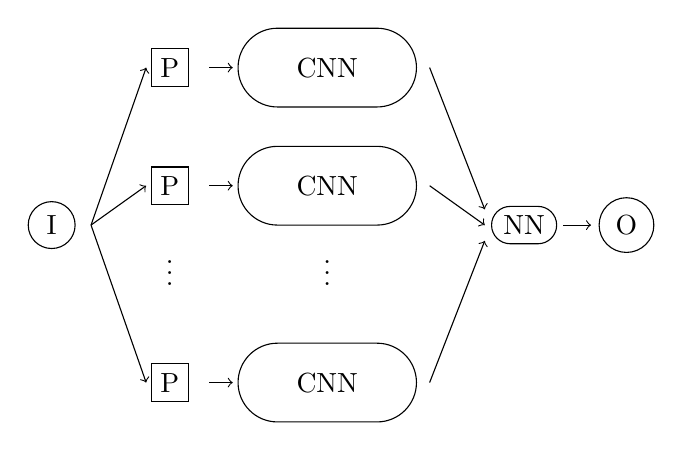
\begin{tikzpicture}
            % image
            \node[circle, draw] (input) at (0,0) {I};
    
            % preprocessed image
            \node[rectangle, draw] (p1) at ($(input) + (1.5,2)$) {P};
            \node[rectangle, draw] (p2) at ($(input) + (1.5,.5)$) {P};
            \node (p3) at ($(input) + (1.5,-.5)$) {\vdots};
            \node[rectangle, draw] (p4) at ($(input) + (1.5,-2)$) {P};
    
            % image to preprocessed image
            \draw[->] ($(input) + (0.5, 0)$) -- ($(p1) + (-0.3, 0)$);
            \draw[->] ($(input) + (0.5, 0)$) -- ($(p2) + (-0.3, 0)$);
            \draw[->] ($(input) + (0.5, 0)$) -- ($(p4) + (-0.3, 0)$);
    
            % cnn
            \node[rounded rectangle, draw, minimum width=2.5cm, minimum height=1cm] (cnn1) at ($(p1) + (2,0)$) {CNN};
            \node[rounded rectangle, draw, minimum width=2.5cm, minimum height=1cm] (cnn2) at ($(p2) + (2,0)$) {CNN};
            \node[minimum width=2.5cm, minimum height=1cm] (cnn3) at ($(p3) + (2,0)$) {\vdots};
            \node[rounded rectangle, draw, minimum width=2.5cm, minimum height=1cm] (cnn4) at ($(p4) + (2,0)$) {CNN};
    
            % preprocessed to cnn
            \draw[->] ($(p1) + (0.5, 0)$) -- ($(cnn1) + (-1.2, 0)$);
            \draw[->] ($(p2) + (0.5, 0)$) -- ($(cnn2) + (-1.2, 0)$);
            \draw[->] ($(p4) + (0.5, 0)$) -- ($(cnn4) + (-1.2, 0)$);
    
            % classifier
            \node[rounded rectangle, draw] (classifier) at ($(cnn3) + (2.5,0.5)$) {NN};
    
            % cnn to classifier
            \draw[->] ($(cnn1) + (1.3, 0)$) -- ($(classifier) + (-.5, .2)$);
            \draw[->] ($(cnn2) + (1.3, 0)$) -- ($(classifier) + (-.5, 0)$);
            \draw[->] ($(cnn4) + (1.3, 0)$) -- ($(classifier) + (-.5, -.2)$);
    
            % output
            \node[circle, draw] (output) at ($(classifier) + (1.3,0)$) {O};
    
            % classifier to output
            \draw[->] ($(classifier) + (.5, 0)$) -- ($(output) + (-.45, 0)$);
    
        \end{tikzpicture}
        \caption{General structure of a MC-CNN.}\label{fig:mc-cnn}
    \end{figure}
    \par{
        The ROIs are then fed into the third part of the proposed architecture, the \emph{classifier}, and properly classified as flawless or flawed; in the latter case, they are assigned a defect class. The \emph{classifier} is structured as a MC-CNN, which in general has the structure illustrated in \emph{Figure \ref{fig:mc-cnn}}. 
    }
    \par{
        First, the input image I is preprocessed to extract $n$ column input P. Second, these P are fed into different CNNs in parallel, therefore all the columns are independent one another. Finally, the output of the MC-CNN columns is combined through a classifier, e.g. a neural network (NN), to produce the final output.
    }
    \par{
        The choice of using a MC-CNN is due to several reasons, beyond the proved effectiveness described in \cite{ieee:6248110}. Primarily, the training of a MC-CNN is highly parallelizable, indeed the different columns can learn separately one from another, once their correspective input is prepared.
    }
    \par{
        Moreover, it is possible to merge both local and global information in a far easier way then using a traditional, single-column, CNN. Indeed, instead of focusing only on a rectangular area, which brings only the local information about the plausible defect, with a MC-CNN it is immediate to add another column concerned with the whole image.
    }
    \par{
        This is the main point in favour of MC-CNN, since the class of a defect may be inferred using global patterns, such as the number of similar areas on the same surface. Imagine, for example, an error burst on the surface. Although traditional single-column CNNs may consider directly the input to the global column, this would face problems regarding the presence of multiple defects classes on the same surface. Therefore, a MC-CNN approach with some columns concerning local information and other focusing on global patterns is heuristically better.
    }
    \par{
        In \emph{Section \ref{section:further-work}} another approach to combine such information through a CNN is described. Although possible, is patently more convoluted then the MC-CNN approach. It would still be interesting to compare them in order to better evaluate the effectiveness of the proposed architecture. 
    }
    \par{
        Observe that the output of the \emph{global column} must be calculated only once per each image, since it is constant throughout the single surface, and, thus, both the training and the predicting process can be lighten.
    }
    \par{
        Finally, as an incidental outcome, it is possible to further study the amount of contribution of the different columns in accurately determining the defective class, if any, of the considered area. These considerations are reported in \emph{Section \ref{section:results}}.
    }
    \par{
        The proposed MC-CNN has three columns, namely a \emph{shape}, a \emph{local} and a \emph{global} column.
    }
    \par{
        The \emph{classifier} was implemented before the \emph{detector}. In fact, although the former relies on the latter for the ROIs and their relative features (described in \emph{Section \ref{section:shape-column}}, \emph{\ref{section:local-column}} and \emph{\ref{section:global-column}}), it was preempting supposed to have an ideal \emph{detector}, i.e. one which proposes the optimal ROIs.
    }
    \par{
        This effort-outcome oriented approach was done for two main reasons. Firstly, it highlights the upper bound reachable with the whole architecture. Secondly, dividing the \emph{detector} outcome from the \emph{classifier} input during the training allows to export the trained MC-CNN and to use it within the challenger architecture, proposed in \emph{Section \ref{section:further-work}}.
    }
    \par{
        The three columns share the common ideas used in edge-cutting work \cite{stanford:cs231n} in their structure, beside some their idiosyncrasies. These are explained in \emph{Section \ref{section:shape-column}}, \emph{\ref{section:local-column}} and \emph{\ref{section:global-column}}.
    }
    \par{
        The basic principles used in structuring the CNNs are mainly three:
        \begin{enumerate}
            \item The input layer should be a multiple of a high power of $2$. Common dimensions are $32$ (e.g. CIFAR-10), $64$, $96$ (e.g. STL-10), or $224$ (e.g. common ImageNet ConvNets), $384$, and $512$. However, the approach described in this paper deals with input images of various size.
            \item The convolutional layers should involve small filters (e.g. $3\times 3$ or $5\times5$), using a unitary stride, and it should not alter the spatial dimensions of the input. Hence, proper padding (e.g., $\left[1,1,1,1\right]$ for $3\times 3$ filters) should be added.
            \item The reduction of the size of the input should be due to the pooling layers, tipically a $2\times 2$ downsampling with a $2\times 2$ stride.
        \end{enumerate}
    }
    \subsection{Shape column}\label{section:shape-column}
        \par{
            The \emph{shape column} is concerned to learn from the shape of the proposed region. This is fed into the CNN as a binary matrix, in which ones represent points in the border of the area.
        }
        \begin{figure}
            \centering
            \includegraphics[width=\linewidth]{graphics/architecture/mc-cnn-shape}
            \vskip 0.05cm
            \includegraphics[width=\linewidth]{graphics/architecture/mc-cnn-shape-filled}
            \caption{Shape column input (top) and filled input (bottom).}\label{fig:mc-cnn:shape-input}
        \end{figure}
        \par{
            An example of this binary images is given in \emph{Figure \ref{fig:mc-cnn:shape-input}} (top). The shape is centered in a $1600\times 256$ black image. Indeed, the size of the input is set to the largest area that could be found, i.e. a defect spanning over the entire surface. The shape is centered to ensure that the classifier is translation independent. 
        }
        \par{
            The \emph{detector}, since is not ideal, provides to the \emph{classifier} also false positive ROIs, i.e. regions that are not defective. Therefore, this stage of the architecture need to be able to discard flawless proposed regions.
        }
        \par{
            However, training the \emph{shape column} to classify some shapes as not defective is not feasible. Indeed, there is not a flawless surface shape, and manually generating it would not be safe.
        }
        \par{
            Hence, the \emph{shape column} should only be trained to classify a region into one of the four defect classes, and to mark flawless proposals will be duty of the final classifier (\emph{Section \ref{section:final-classifier}}).
        }
        \par{
            Therefore, the output layer is a $n$-dimensional vector, where $n$ is the number of defect classes. Each entry of this vector describes the confidence of the network in considering the input shape as related to one of the $n$ defect classes.
        }
        \par{
            However, from data analysis was observed that, sometimes, defective input defects of the same class are clustered together, since very near one another. This is usually true for defects of class No.3, which are burst defects and might be nearly adjacent. Therefore, the shape that would be extracted is the shape of the region and not the one of the defects. Hence, the network would not be properly trained.
        }
        \par{
            For this reason, the \emph{shape column} is left as a further development in \emph{Section \ref{section:further-work}}.
        }
        \par{
            The \emph{shape column} input could also be filled before to be fed into the CNN, as shown in \emph{Figure \ref{fig:mc-cnn:shape-input}} (bottom).
        }
    \subsection{Local column}\label{section:local-column}
        \par{
            The \emph{local column} is thought to consider luminance levels around the border of the defect, to learn from the local context. Similarly to the \emph{shape column} (\emph{Section \ref{section:shape-column}}), this column is concerned only in classifying proposals into one of the four defective classes.
        }
        \begin{figure}
            \centering
            \includegraphics[width=\linewidth]{graphics/architecture/mc-cnn-local}
            \caption{Local column input.}\label{fig:mc-cnn:local-input}
        \end{figure}
        \par{
            Therefore, the column is fed with the grey scale portion of the image inside the bounding box of the considered region. As an example, in \emph{Figure \ref{fig:mc-cnn:local-input}} is illustrated a plausible input to the \emph{local column}.
        }
        \par{
            This grey scale portion is generated from the shape of the region and the original image.
        }
        \par{
            Firstly, the bounding box of the shape is calculated. Secondly, the original image outside the bounding box is discarded. Finally, the cropped image is centered in a black $1600\times 256$ picture. The reasons behind the centering and the dimensioning of the input are the same described in \emph{Section \ref{section:shape-column}}.
        }
        \begin{table*}
            \centering
            \normalsize
            \begin{tabular}{|l|l|l|l|}
                \hline
                    \textbf{Layer} & \textbf{Type} & \textbf{Activations} & \textbf{Learnables}\\\hline
                    Input & Image input & $256\times 1600 \times 1 = 409.600$ & \\
                    $\left[256\times 1600\times 1\right]$ image & & & \\
                    ``zerocenter'' normalization & & & \\\hline
                    %%%%
                    Spreader & Convolution & $800\times 800\times 4 = 2.560.000$ & Weights $3\times 3\times 1 \times 4 = 36$\\
                    Filter $4$ $\left[3\times 3\times 1\right]$ & & & Bias $1\times 1\times 4 = 4$\\
                    Stride $\left[1\;1\right]$ & & & Total: $40$ \\
                    Dilation factor $\left[400\;400\right]$ & & & \\
                    Padding $\left[672\;0\right]$ & & & \\\hline
                    %%%%
                    Conv1 & Convolution & $800\times 800\times 8 = 5.120.000$ & Weights $3\times 3\times 4 \times 8 = 288$\\
                    Filter $8$ $\left[3\times 3\times 4\right]$ & & & Bias $1\times 1\times 8 = 8$\\
                    Stride $\left[1\;1\right]$ & & & Total: $296$\\
                    Padding ``same'' & & & \\\hline
                    %%%%
                    MaxPool1, $\left[4\times 4\times 1\right]$ & Max pooling & $200\times 200\times 8 = 320.000$ & \\
                    Stride $\left[4\;4\right]$ & & & \\
                    Padding ``same'' & & & \\\hline
                    %%%%
                    Conv2 & Convolution & $200\times 200\times 16 = 640.000$ & Weights $3\times 3\times 8 \times 16 = 1152$\\
                    Filter $16$ $\left[3\times 3\times 8\right]$ & & & Bias $1\times 1\times 16 = 16$\\
                    Stride $\left[1\;1\right]$ & & & Total: $1168$\\
                    Padding ``same'' & & & \\\hline
                    %%%%
                    MaxPool2, $\left[4\times 4\times 1\right]$ & Max pooling & $50\times 50\times 16 = 40.000$ & \\
                    Stride $\left[4\;4\right]$ & & & \\
                    Padding ``same'' & & & \\\hline
                    %%%%
                    Conv3 & Convolution & $50\times 50\times 32 = 640.000$ & Weights $3\times 3\times 16 \times 32 = 4.608$\\
                    Filter $32$ $\left[3\times 3\times 16\right]$ & & & Bias $1\times 1\times 32 = 32$\\
                    Stride $\left[1\;1\right]$ & & & Total: $4640$\\
                    Padding ``same'' & & & \\\hline
                    %%%%
                    MaxPool3, $\left[2\times 2\times 1\right]$& Max pooling & $25\times 25\times 32 = 20.000$ & \\
                    Stride $\left[2\;2\right]$ & & & \\
                    Padding ``same'' & & & \\\hline
                    %%%%
                    Conv4 & Convolution & $25\times 25\times 64 = 40.000$ & Weights $3\times 3\times 32 \times 64 = 18.432$\\
                    Filter $64$ $\left[3\times 3\times 32\right]$ & & & Bias $1\times 1\times 64 = 64$\\
                    Stride $\left[1\;1\right]$ & & & Total: $18496$\\
                    Padding ``same'' & & & \\\hline
                    %%%%
                    MaxPool4, $\left[2\times 2\times 1\right]$ & Max pooling & $13\times 13\times 64 = 10.816$ & \\
                    Stride $\left[2\;2\right]$ & & & \\
                    Padding ``same'' & & & \\\hline
                    %%%%
                    Conv5 & Convolution & $13\times 13\times 128 = 21.632$ & Weights $3\times 3\times 64 \times 128 = 73.728$\\
                    Filter $128$ $\left[3\times 3\times 64\right]$ & & & Bias $1\times 1\times 128 = 128$\\
                    Stride $\left[1\;1\right]$ & & & Total: $73856$\\
                    Padding ``same'' & & & \\\hline
                    %%%%
                    MaxPool5, $\left[2\times 2\times 1\right]$ & Max pooling & $7\times 7\times 128 = 6.272$ & \\
                    Stride $\left[2\;2\right]$ & & & \\
                    Padding ``same'' & & & \\\hline
                    %%%%
                    FullConn1 & Fully connected & $1\times 1\times 16 = 16$ & Weights $16\times 6272 = 100.352$\\
                    & & & Bias $16\times 1 = 16$\\
                    & & & Total: $100.368$\\\hline
                    %%%%
                    FullConn2 & Fully connected & $1\times 1\times 16 = 16$ & Weights $16\times 16 = 256$\\
                    & & & Bias $16\times 1 = 16$\\
                    & & & Total: $272$\\\hline
                    %%%%
                    FullConn3 & Fully connected & $1\times 1\times 4 = 4$ & Weights $4\times 16 = 64$\\
                    & & & Bias $4\times 1 = 4$\\
                    & & & Total: $68$\\\hline
                    %%%%
                    Output & Softmax & $1\times 1\times 4 = 4$ & \\
                \hline
            \end{tabular}
            \vspace{0.5cm}
            \caption{Local column CNN layers.}\label{table:mc-cnn:local-structure}
        \end{table*}
        \par{
            The layers of this CNN are shown in \emph{Table \ref{table:mc-cnn:local-structure}}. The output layer is analogous to the one in \emph{Section \ref{section:shape-column}}.
        }
        \par{
            The peculiarity of this CNN lies in its first convolutional layer, named \emph{spreader}. It is a novel application of the dilation factor. 
        }
        \par{
            Recall that given a $n\times n$ filter, a dilation of $[a\;b]$ applied to the given filter produces a $\left[\left(n-1\right)*a + 1\right] \times \left[\left(n-1\right)*b + 1\right]$ filter. The original entries are equally spreaded in the new filter, whereas the additional values are null.
        }
        \par{
            As an example, the below transformation applies a dilation factor of $\left[3\;5\right]$ to the given $2\times 2$ filter.
        }
        \begin{BVerbatim}
            
                          _           _
     _   _               | a 0 0 0 0 b |
    | a b |   [3 5]      | 0 0 0 0 0 0 |
    | c d |  ------>     | 0 0 0 0 0 0 |
     -   -               | c 0 0 0 0 d |
                          -           -
                    
        \end{BVerbatim}
        \par{
            An example on a $3\times 3$ filter is proposed below:
        } 
        \begin{BVerbatim}
            
                            _         _
     _     _               | a 0 b 0 c |
    | a b c |   [2 2]      | 0 0 0 0 0 |
    | d e f |  ------>     | d 0 e 0 f |
    | g h i |              | 0 0 0 0 0 |
     -     -               | g 0 h 0 i |
                            -         -
                    
        \end{BVerbatim}
        \par{
            The dilation factor is usually used in CNNs to implement a wider receptive field, using the same number of weights. Indeed, a $K_1 \times K_2$ filter convolves pixels in an area of $K_1 \times K_2$. Using a dilation factor of $\left[a\;b\right]$ it would convolve the same number of pixels, but on an area of $\left[\left(K_1-1\right)*a + 1\right] \times \left[\left(K_2-1\right)*b + 1\right]$. Using a proper stride, this would be the same of a downsampling followed by a convolution.
        }
        \par{
            However, in the proposed architecture it is used in a novel way, to address the problem of different-sized bounding boxes. In fact, the usage of the \emph{spreader} layer aims to reproduce in different locations of the layer activation the original informative region, through some learned linear functions. Indeed, with a proper sizing, the convolution in the first layer results in the sum of the bias factor and a single informative pixel multiplied by a weight of the filter.
        }
        \begin{figure}
            \centering
            \includegraphics[width=\linewidth]{graphics/architecture/act_net}
            \vskip .05cm
            \includegraphics[width=\linewidth]{graphics/architecture/act_net_hope}
            \caption{Learned features with a traditional convolutional layer (top) and with the \emph{spreader} (bottom). $4$ tiled features are illustrated in both cases.}\label{fig:learned-features-hope-net}
        \end{figure}
        \par{
            In \emph{Figure \ref{fig:learned-features-hope-net}} the learned features of four $3\times3$ filters of a traditional convolutional layer with padding $\left[673\;1\right]$ are juxtaposed to the ones learned by four $3\times 3$ filters with a dilation factor of $\left[400\;400\right]$ and proper padding $\left[672\;0\right]$. 
        }
        \par{
            The two pictures are scaled to be paired. However, the former is $1600 \times 1600$, the latter is $800\times 800$. Still it is patent that the proposed approach greatly exceed the traditional one in terms of information kept. 
        }
        \par{
            Indeed, the problem with convolutional layer with massive padding (in alternative to cropping) is that large empty regions have null activations. Then, pooling layers keep the proportions between \emph{death} area and the informative, central, region. This leads to massive memory waste.
        }
        \par{
            A $3\times 3$ filter with a dilation factor of half the output activation size and proper padding enhances the effectiveness of the following layers, recycling empty areas. In fact, they are convolved together with the central informative region.
        }
        \par{
            Indeed, this approach ensures that at least $9$ areas will convolve with the central region. The learned weights of the filter will then decide whether to copy, along with some multiplicative factor (which can be thought as varying the exposure of the image portion), the defect in these new regions.
        }
        \par{
            Therefore, without any manual tuning, the network would eventually learn to handle large original pictures. As an example, if the dataset is composed by a cornucopia of large defects, the \emph{spreader} may copy only vertically the defect, using only three of the nine available weights.
        }
        \par{
            In the proposed architecture, four of this spreading filters are used in the first layer, conceptually in order to tune them one per defective class.
        }
        \par{
            The \emph{spreader} layer represents an effective alternative to either lossy crop or padding when dealing with either images of different dimensions or non-squared pictures.
        }
        \par{
            By cropping the image, massive memory saving could be allowed. As an example, the $512\times 512$ cropping proposed in \emph{Table \ref{table:cropping}} would save $800\times 800 - 512\times 512 \approx \SI{1}{\mega\byte}$ per image, about $59.04\%$.
        }
        \par{
            However, the proposed spreader introduces $\times 9$ information compared to cropping, which is followed by activations similar, although with less memory consumption, to the ones shown in \emph{Figure \ref{fig:learned-features-hope-net}} (top).
        }
        \par{
            There is patently a tradeoff between training time, memory (hence both batch and mini-bath size), number of weights and information loss.
        }
        \par{
            Using a classical approach with these different-sized bounding boxes, with either cropping or padding, would conceptually lead at the end to suppress informative areas, due both to pooling and convolving empty regions.
        }
        \begin{figure}
            \centering
            \begin{subfigure}{.5\linewidth}
                \centering
                \includegraphics[width=.9\linewidth]{graphics/architecture/act_net_out}
                % \caption{}
            \end{subfigure}\hfill
            \begin{subfigure}{.5\linewidth}
                \centering
                \includegraphics[width=.9\linewidth]{graphics/architecture/act_net_hope_out}
                % \caption{}
            \end{subfigure}
            \caption{Final layer features with classical architecture ($512$ $13\times 13$ features) (a) and with the spreader ($128$ $13\times 13$ features) (b).}
            \label{fig:features-last-layer}
        \end{figure}
        \par{
            Instead, the proposed initial layer spreads over the squared activation matrix the defect, allowing to have more informative features in the final layer, as visible in the comparison in \emph{Figure \ref{fig:features-last-layer}}. Indeed, the visual effect of equivalence between the two suggests that the initial \emph{spreader} reduces the number of successive filters required, hence the number of parameters. A smaller number of parameters requires less data to prevent overfitting. If the outcomes are the same, it means that the model is better.
        }
        \par{
            What can be heuristically inferred is that what is lost as memory efficiency, is far more gained as information. Hence, the memory can be saved in successive layers of the architecture. In the proposed architecture this is done through the first two max pooling layers, each of them introducing a shrinking factor of $4$.
        }
        \par{
            Moreover, performing a massive crop operation one accepts to misclassify a given percentage of the dataset. From an intuitive point of view, the \emph{spreader} could learn to repeat the defect only vertically.
            For example, the filter:
        }
        \par{
        \begin{BVerbatim}

            _     _
           | 1 0 0 |
           | 1 0 0 |
           | 1 0 0 |
            -     -
       \end{BVerbatim}
        }
        \par{
            would simply replicate three times the image vertically. The takeaway is that this filter removes the manual tuning of the crop operation, while it improves the efficiency of the feature extraction stage of the CNN.
        }
        \par{
            However, further investigating the effectiveness of the \emph{spreader}, compared to the crop operation, is proposed in \emph{Section \ref{section:further-work}}.
        }
    \subsection{Global column}\label{section:global-column}
        \begin{figure}
            \centering
            \includegraphics[width=\linewidth]{graphics/architecture/mc-cnn-global}
            \caption{Global column input.}\label{fig:mc-cnn:global-input}
        \end{figure}
        \par{
            The \emph{global column} is concerned in detecting global patterns, such as zipper cracks. Hence, it is fed with the whole image. An example of input is shown in \emph{Figure \ref{fig:mc-cnn:global-input}}. The importance of this column is clear from the observations made in \emph{Section \ref{subsection:defects}}. Indeed, when two different classes are locally equal, the \emph{global column} is determinant to correctly classify the defective region.
        }
        \par{
            Ideally, the \emph{global column} should output a $16$-dimensional vector, with one entry per combination of classes. However, the dataset is very skewed when accounting for different classes combinations, as illustrated in \emph{Figure \ref{fig:defects:combinations}}. Hence, the output layer has to be structured in a different way. Moreover, the inner structure of the CNN should be deeper then the other two, and, thus, requires a larger amount of data. Since longer training times and more hardware resources are required, the \emph{global column} is left as a further development in \emph{Section \ref{section:further-work}}.
        }
    \subsection{Final classifier}\label{section:final-classifier}
        \par{
            The outcomes of the different columns of a MC-CNN are then combined to obtain the final output. In the proposed architecture, this combination is done through a neural network, since a manual tuning of such data fusion would be ineffective.
        }
        \begin{figure}
            \centering
            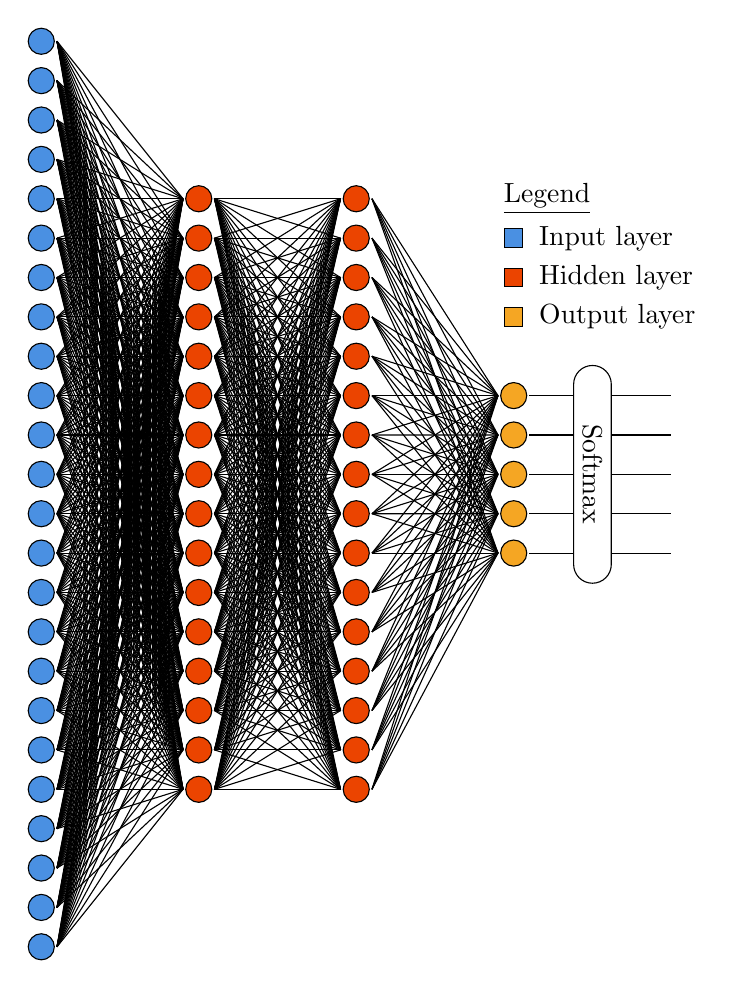
\begin{tikzpicture}
                % input layer
                \foreach \i in {0,...,23}
                    \node[circle, draw, minimum height=1, minimum width=1,fill=blue] (input \i) at (0,-\i*0.5) {};

                % hidden layer
                \foreach \i in {0,...,15}
                    \node[circle, draw, minimum height=1, minimum width=1,fill=orange] (hidden \i) at ($(input 4) + (2,-\i*0.5)$) {};

                % from input to hidden layer
                \foreach \i in {0,...,23}
                    \foreach \j in {0,...,15}
                        \draw ($(input \i) + (.2,0)$) -- ($(hidden \j) + (-.2,0)$);

                % hidden layer 2
                \foreach \i in {0,...,15}
                    \node[circle, draw, minimum height=1, minimum width=1,fill=orange] (hidden 2 \i) at ($(hidden 0) + (2,-\i*0.5)$) {};

                % from hidden to hidden layer
                \foreach \i in {0,...,15}
                    \foreach \j in {0,...,15}
                        \draw ($(hidden \i) + (.2,0)$) -- ($(hidden 2 \j) + (-.2,0)$);

                % output layer
                \foreach \i in {0,...,4}
                    \node[circle, draw, minimum height=1, minimum width=1,fill=yellow] (output \i) at ($(hidden 2 5) + (2,-\i*0.5)$) {};

                % from hidden 2 to output layer
                \foreach \i in {0,...,15}
                    \foreach \j in {0,...,4}
                        \draw ($(hidden 2 \i) + (.2,0)$) -- ($(output \j) + (-.2,0)$);

                % from output to softmax layer
                \foreach \i in {0,...,4}
                    \draw ($(output \i) + (.2,0)$) -- ($(output \i) + (2,0)$);

                % softmax layer
                \node[rounded rectangle, fill=white, minimum width=3cm,draw,rotate=-90] (softmax) at ($(output 2) + (1,0)$) {Softmax};

                % legend
                \node[rectangle, draw, fill=yellow, minimum width=1, minimum height=1] (output label color) at ($(output 0) + (0,1)$) {};
                \node[anchor=west] (output label) at ($(output label color) + (.2,0)$) {Output layer};

                \node[rectangle, draw, fill=orange, minimum width=1, minimum height=1] (hidden label color) at ($(output label color) + (0,.5)$) {};
                \node[anchor=west] (hidden label) at ($(hidden label color) + (.2,0)$) {Hidden layer};

                \node[rectangle, draw, fill=blue, minimum width=1, minimum height=1] (input label color) at ($(hidden label color) + (0,.5)$) {};
                \node[anchor=west] (input label) at ($(input label color) + (.2,0)$) {Input layer};

                \node[anchor=west] (legend label) at ($(input label color) + (-.25,.5)$) {\underline{Legend}};
            \end{tikzpicture}
            \caption{Final classifier structure.}\label{fig:mc-cnn:final-classifier-structure}
        \end{figure}
        \par{
            In \emph{Figure \ref{fig:mc-cnn:final-classifier-structure}} the structure of the last layer of the architecture is described. The first layer is constrained to the output size of the three columns, i.e. $4+4+16 = 24$. Then there are two hidden layers with $16$ activation units, and finally the output layer with $5$ neurons. The output is passed through a softmax layer, hence the final output describe the confidence per each class and for the flawless regiono condition.
        }
        \par{
            Observe that bias units have not been included in the picture.
        }
        \par{
            The \emph{final classifier} is left as further work, together with both \emph{shape} and \emph{global columns}, in \emph{Section \ref{section:further-work}}.
        }

    % Challenger
    % \section{Challengers}\label{section:challengers}
    \par{
        .... exaplain the need for challengers
    }
    \subsection{Sliding window}
        \par{
            ... exaplain briefly the approach
        }
        \par{
            ... image pyramids
        }

    \subsection{Landmarks}
        \par{
            ... explain briefly the approach
        }

    \subsection{Thresholding and location aggregation}
        \par{
            ... In both cases segmentation is needed ...
            .... Explain how from confidence value on different region of interests one can build the localization of defects area ....
        }
    % Results
    \section{Results}\label{section:results}
    Review the article, make some considerations on results and provide suggestions to further work...

    *** Confronto con esplicitamente indicati il contributo di ogni step al miglioramento del risultato ***

    The whole system implementation can be found in the \href{https://github.com/antonioterpin/wavelet_ml}{\texttt{GitHub}} repository \cite{antonioterpin:github}.

    % \begin{table}
    %     \caption{TODO RESULTS WITH SOME METRICS}
    % \end{table}
    % \input{sections/acknowledgment.tex}

    % \appendices
    
    \bibliographystyle{IEEEtran}
    \bibliography{references}

\end{document}

